\chapter{Desarrollo de la Solución}

\section{Operacionalización de variables}
Donde:
\begin{itemize}
    \item TP (True Positives): Casos correctamente clasificados como positivos.
    \item TN (True Negatives): Casos correctamente clasificados como negativos.
    \item FP (False Positives): Casos incorrectamente clasificados como positivos.
    \item FN (False Negatives): Casos incorrectamente clasificados como negativos.
\end{itemize}

\begin{figure}
    \centering
    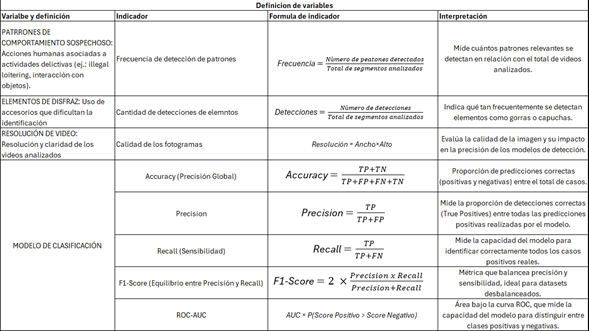
\includegraphics[width=1.1\linewidth]{4/op var.png}
\end{figure}
\clearpage

\section{Técnicas de Recolección de Datos}
La recolección de datos para esta investigación se basa en la obtención de videos de vigilancia provenientes de cámaras municipales en zonas urbanas de alto riesgo en Lima, Perú. Este proceso comienza con la identificación de áreas prioritarias, utilizando reportes estadísticos y policiales que reflejan las zonas con mayor incidencia delictiva. Una vez seleccionadas estas áreas, se identifican las cámaras municipales disponibles en dichas ubicaciones, evaluando su relevancia y calidad como fuente de datos.

Posteriormente, se elabora una solicitud formal dirigida a las municipalidades, explicando los objetivos de la investigación y detallando las especificaciones de los datos requeridos. Estas solicitudes garantizan el cumplimiento de normativas de privacidad y confidencialidad. Una vez enviadas, se realiza un seguimiento para negociar términos de acceso que permitan la utilización de los videos con fines investigativos.

Tras la recepción de los videos, estos son revisados para asegurar que cumplan con los estándares técnicos necesarios, como el formato (MP4 o AVI) y una resolución mínima de 720p. Este proceso asegura que los datos recolectados sean útiles y de calidad suficiente para entrenar los modelos de inteligencia artificial diseñados para detectar comportamientos sospechosos. Finalmente, los videos se preparan para el análisis, asegurando que estén listos para su preprocesamiento y segmentación en fragmentos relevantes.

\begin{figure}[h] % "h" indica que la imagen se coloque aproximadamente aquí
    \centering
    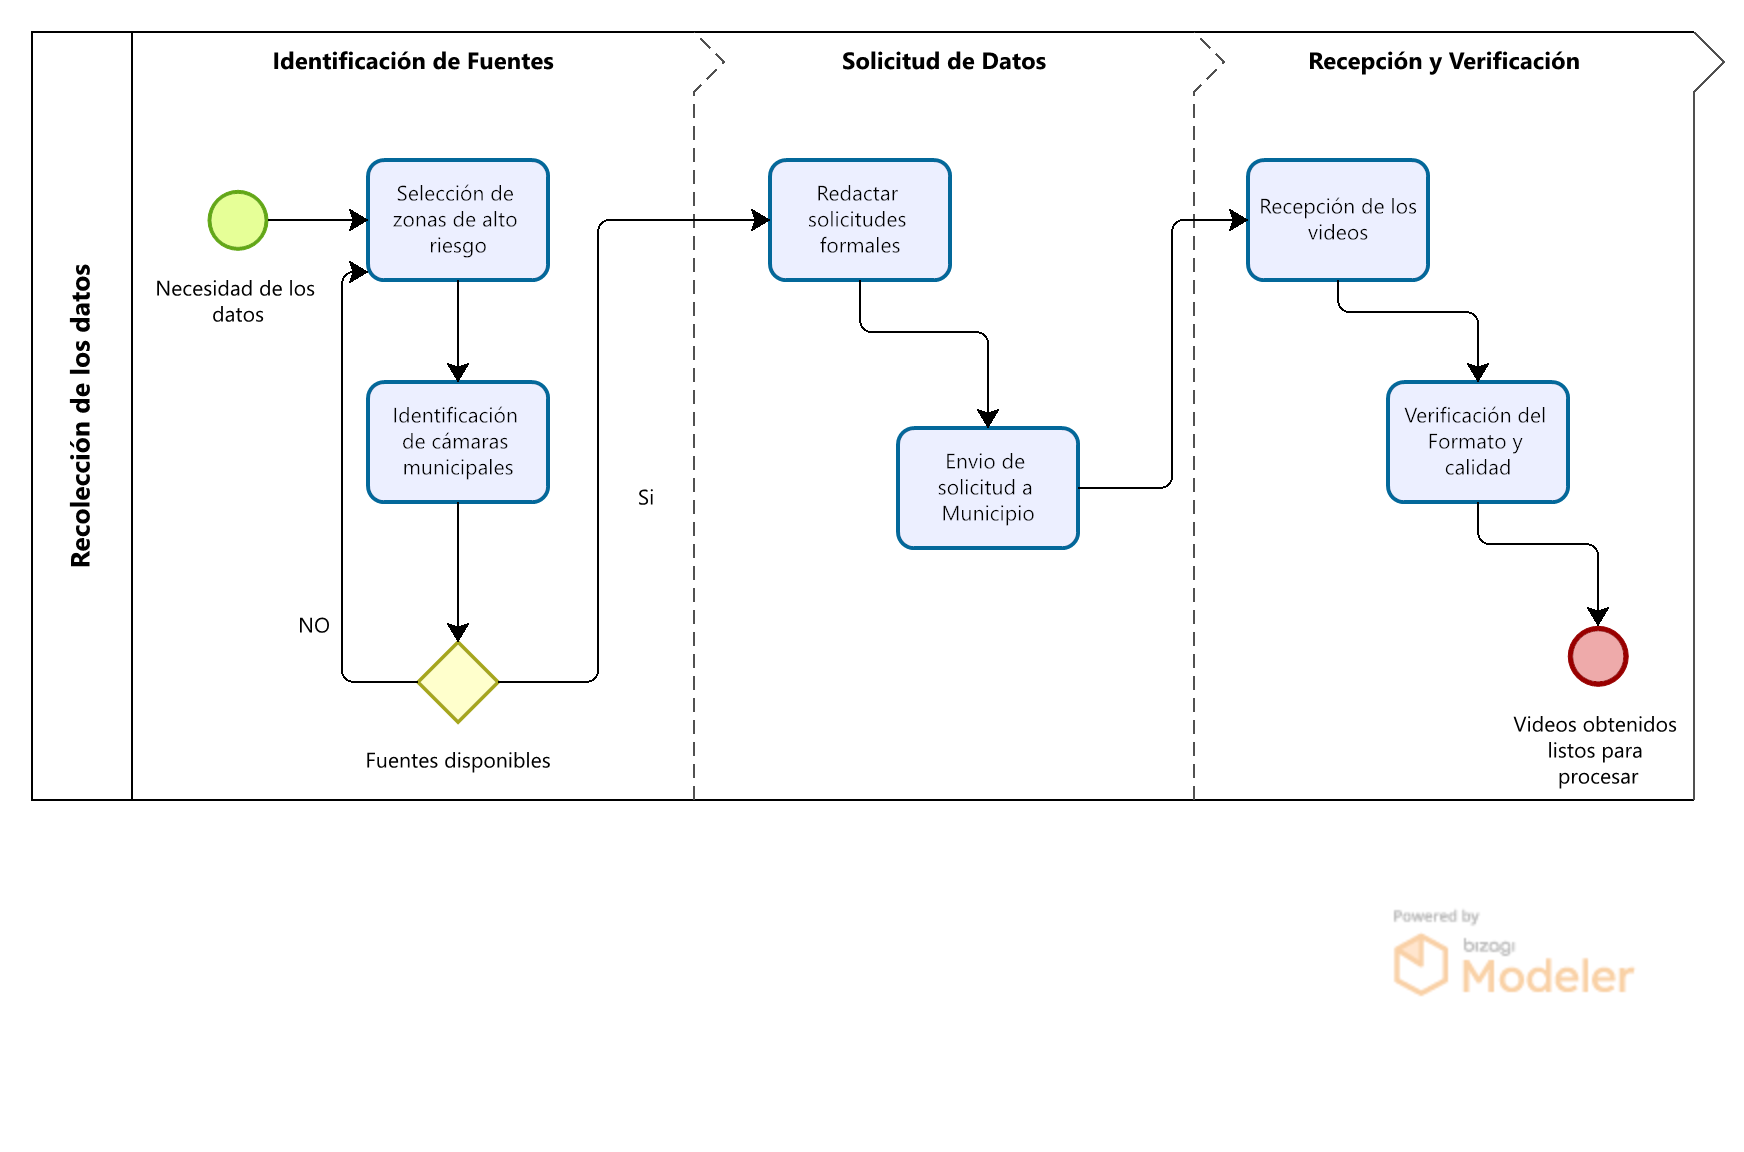
\includegraphics[width=1.0\textwidth]{4/Flujograma data.png} % Ruta y tamaño de la imagen
    \label{fig:ejemplo} % Etiqueta para referenciar la imagen
\end{figure}

\section{Técnicas para el Procesamiento y Análisis de la Información}
Para abordar el problema de la detección de comportamientos sospechosos en entornos urbanos, se seleccionó una metodología basada en los antecedentes más relevantes de la literatura científica. Los estudios de Sultani et al. (2018), Sun et al. (2021), y otros autores han demostrado la eficacia de enfoques híbridos que combinan aprendizaje profundo, extracción de características y segmentación en tiempo real para analizar datos visuales en entornos de vigilancia. Esta investigación adapta y expande estas metodologías para optimizar la precisión y robustez del sistema propuesto.


\begin{figure}[h] % "h" indica que la imagen se coloque aproximadamente aquí
    \centering
    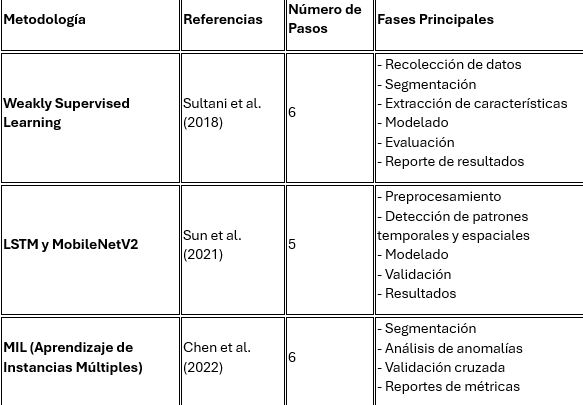
\includegraphics[width=1.0\textwidth]{4/figures/proceso.png} % Ruta y tamaño de la imagen
    \label{fig:ejemplo} % Etiqueta para referenciar la imagen
\end{figure}
\clearpage

Se adaptó un enfoque híbrido basado en Weakly Supervised Learning y técnicas avanzadas de redes neuronales recurrentes para implementar la solución. La elección de esta metodología se fundamenta en su capacidad para manejar grandes volúmenes de datos visuales, adaptarse a escenarios urbanos complejos y proporcionar resultados en tiempo real, como se evidencia en los antecedentes citados.


\begin{figure}[h] % "h" indica que la imagen se coloque aproximadamente aquí
    \centering
    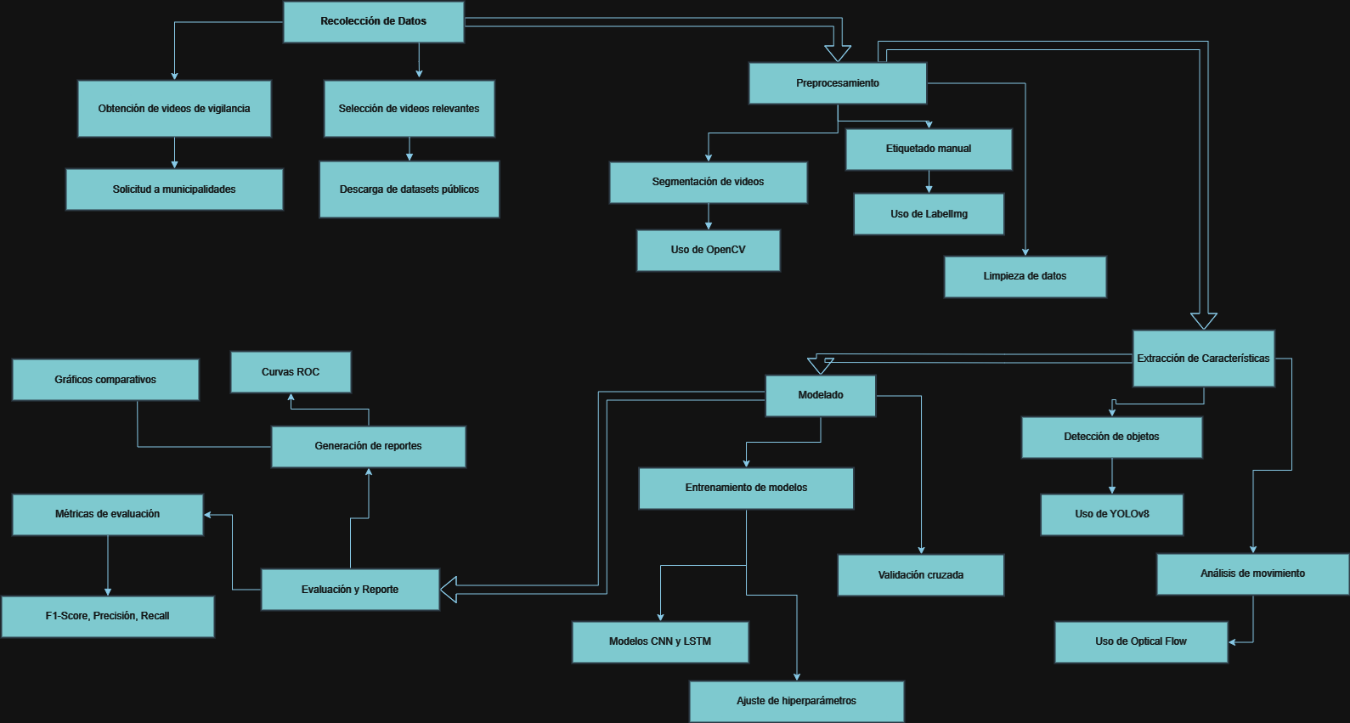
\includegraphics[width=0.8\textwidth]{4/propuesta.png} % Ruta y tamaño de la imagen
    \label{fig:ejemplo} % Etiqueta para referenciar la imagen
\end{figure}

\subsection{Recolección de Datos}
La primera etapa se enfoca en la obtención de videos relevantes para el análisis de comportamientos sospechosos en zonas urbanas de alto riesgo. Los datos se recopilarán de dos fuentes principales:
\begin{itemize}
    \item Cámaras municipales en zonas priorizadas mediante solicitudes formales a las municipalidades.
    \item Datasets públicos relevantes, como UCF-Crime, que contienen videos etiquetados de actividades anómalas.
\end{itemize}
Nuestro objetivo es asegurar una base de datos adecuada en términos de calidad, formato y cantidad, necesaria para el entrenamiento y validación de los modelos de inteligencia artificial.

\paragraph{\textit{Actividades}}

\subsubsection{Identificación de Fuentes}

\begin{itemize}
    \item Definir zonas urbanas de alto riesgo basadas en reportes policiales y estadísticas.
    \item Localizar cámaras municipales y privadas disponibles en esas zonas.
\end{itemize}

\subsubsection{Elaboración de Solicitudes}
\begin{itemize}
    \item Preparar solicitudes formales dirigidas a municipalidades y otras entidades responsables, explicando los objetivos de la investigación y el uso planificado de los videos.
\end{itemize}

\subsubsection{Revisión de Datasets Públicos}
\begin{itemize}
    \item Analizar datasets existentes como UCF-Crime y otros similares para complementar los datos municipales.
    \item Asegurar que los datos cumplan con los requisitos de calidad (formato MP4 o AVI, resolución mínima 720p).
\end{itemize}

\subsubsection{Recepción y Almacenamiento}
\begin{itemize}
    \item Centralizar los videos recolectados en un repositorio seguro.
    \item Organizar los datos por zonas, fechas y relevancia del contenido.
\end{itemize}


\paragraph{\textit{Herramientas Utilizadas}}

\subsubsection{Software}
\begin{itemize}
    \item Google Drive y herramientas similares para almacenamiento temporal.
    \item Excel/Google Sheets para la organización de los metadatos (ubicación, fecha, duración, calidad).
\end{itemize}

\subsubsection{Datasets Públicos}
\begin{itemize}
    \item UCF-Crime Dataset: Incluye videos etiquetados de actividades sospechosas.
\end{itemize}

\paragraph{\textit{Entregables}}

\subsubsection{Base de Datos Consolidada}
\begin{itemize}
    \item Videos organizados por zona y fecha.
    \item Identificación de videos relevantes para el análisis.
\end{itemize}

\subsubsection{Reporte de Calidad de los Datos}
\begin{itemize}
    \item Evaluación inicial de la calidad de los videos (formato, resolución, duración).
    \item Identificación de videos que requieren preprocesamiento adicional.
\end{itemize}



\subsection{Preprocesamiento}
En esta fase, los videos recolectados se preparan para el análisis. Este proceso incluye la limpieza de datos irrelevantes, la segmentación de los videos en fragmentos manejables y el etiquetado manual o semiautomático de eventos relevantes. El objetivo principal es garantizar que los datos estén listos para el entrenamiento de los modelos de inteligencia artificial.
Lo que se busca es optimizar la calidad de los datos y estructurarlos de manera que puedan ser utilizados eficazmente por los algoritmos de aprendizaje profundo.

\paragraph{\textit{Actividades}}

\subsubsection{Limpieza de Datos}

\begin{itemize}
    \item Verificar la resolución de los videos y descartar aquellos con calidad inferior a 720p.
    \item Eliminar segmentos de video que no contengan actividad humana relevante o que presenten problemas técnicos como ruido excesivo.
\end{itemize}


\subsubsection{Segmentación}
\begin{itemize}
    \item Dividir los videos en fragmentos más pequeños (30 segundos a 5 minutos) para facilitar el procesamiento y etiquetado.
    \item Utilizar herramientas como OpenCV para automatizar el proceso de segmentación.
\end{itemize}

\subsubsection{Etiquetado Manual}
Clasificar los fragmentos de video según categorías específicas como
\begin{itemize}
    \item Loitering: Comportamiento de permanencia prolongada.
    \item Interacción con objetos: Manipulación sospechosa de mochilas u otros elementos.
    \item Movimientos repetitivos: Indicativos de evasión o preparación para actividades delictivas.
\end{itemize}

\subsubsection{Normalización de Datos}
Asegurar que todos los videos segmentados tengan un formato estándar (e.g., MP4) y una resolución consistente para evitar problemas en el entrenamiento.


\paragraph{\textit{Herramientas Utilizadas}}

\subsubsection{Software}
\begin{itemize}
    \item OpenCV: Para la segmentación automática de videos.
    \item LabelImg: Para etiquetar manualmente los comportamientos sospechosos.
\end{itemize}

\subsubsection{Hardware}
\begin{itemize}
    \item Computadoras con capacidad para manejar procesamiento intensivo de video.
    \item Almacenamiento seguro para guardar los fragmentos procesados
\end{itemize}

\paragraph{\textit{Entregables}}

\subsubsection{Dataset Segmentado}
\begin{itemize}
    \item Fragmentos de video clasificados y organizados.
    \item Estructura clara para facilitar el acceso y uso en etapas posteriores.
\end{itemize}


\subsubsection{Reporte de Limpieza}
\begin{itemize}
    \item Detalle de los videos descartados y las razones (e.g., baja calidad, ausencia de actividad relevante).
\end{itemize}


\subsubsection{Anotaciones Etiquetadas}
\begin{itemize}
    \item Dataset enriquecido con etiquetas manuales, indicando eventos sospechosos.
\end{itemize}




\subsection{Extracción de Características}

En esta etapa, se identifican patrones visuales y temporales relevantes de los videos segmentados y etiquetados. Esto incluye analizar aspectos como la detección de objetos, trayectorias de movimiento y comportamientos anómalos. La extracción de características permite transformar los datos visuales en variables cuantificables que serán utilizadas en los modelos de aprendizaje.
El extraer información clave de los videos procesados es fundamental para optimizar el desempeño de los modelos de clasificación y predicción.


\paragraph{\textit{Actividades}}

\subsubsection{Análisis Visual}

\begin{itemize}
    \item Detectar objetos relevantes como gorras, capuchas o mochilas utilizando algoritmos avanzados como YOLOv8.
    \item Identificar posturas corporales sospechosas que puedan indicar comportamientos delictivos.
\end{itemize}


\subsubsection{Análisis Temporal}
\begin{itemize}
    \item Evaluar trayectorias de movimiento mediante Optical Flow para identificar patrones anómalos, como movimientos repetitivos o evasivos.
    \item Analizar la interacción entre individuos o con objetos en el espacio monitoreado.
\end{itemize}


\subsubsection{Conversión de Datos}
\begin{itemize}
    \item Transformar las características visuales y temporales extraídas en variables tabulares para su posterior uso en algoritmos de clasificación.
    \item Estandarizar los valores obtenidos para garantizar consistencia en el entrenamiento de los modelos.
\end{itemize}



\subsubsection{Validación de Características}
\begin{itemize}
    \item Realizar un análisis exploratorio de las características extraídas para verificar su relevancia y eliminar variables redundantes o no significativas.
\end{itemize}


\paragraph{\textit{Herramientas Utilizadas}}

\subsubsection{Software}
\begin{itemize}
    \item YOLOv8: Para la detección de objetos en tiempo real.
    \item Optical Flow: Para el análisis de movimientos en secuencias de video.
\end{itemize}

\subsubsection{Hardware}
\begin{itemize}
    \item GPU de alto rendimiento para acelerar los procesos de detección y análisis.
\end{itemize}

\paragraph{\textit{Entregables}}

\subsubsection{Dataset de Características}
\begin{itemize}
    \item Archivo tabular con las variables clave extraídas de los videos (e.g., número de objetos detectados, trayectorias de movimiento).
\end{itemize}

\subsubsection{Reporte de Análisis Exploratorio}
\begin{itemize}
    \item Resumen estadístico y visualización inicial de las características más relevantes.
\end{itemize}

\subsubsection{Variables Estandarizadas}
\begin{itemize}
    \item Conjunto de datos listo para el modelado, con valores normalizados y sin redundancias.
\end{itemize}


\subsection{Modelado}
Esta etapa se centra en la implementación de modelos de aprendizaje profundo y supervisado para la detección de comportamientos sospechosos. Utilizando características visuales y temporales extraídas en la fase previa, se entrenan y validan los modelos para garantizar que puedan identificar patrones sospechosos con alta precisión.
Lo que buscamos es diseñar y entrenar modelos robustos de aprendizaje que permitan analizar datos de vigilancia en tiempo real y emitir alertas precisas.


\paragraph{\textit{Actividades}}

\subsubsection{Selección de Modelos}

\begin{itemize}
    \item YOLOv8: Para la detección en tiempo real de objetos y posturas corporales.
    \item ConvLSTM: Para analizar secuencias temporales y detectar patrones anómalos.
    \item SVM (Support Vector Machines): Para clasificar eventos específicos con características predefinidas como gorras o movimientos repetitivos.
\end{itemize}


\subsubsection{Configuración del Entorno}
\begin{itemize}
    \item Frameworks como TensorFlow y PyTorch.
    \item Configuración de GPU para acelerar el entrenamiento.
\end{itemize}


\subsubsection{Entrenamiento de los Modelos}
Dividir el dataset en:
\begin{itemize}
    \item 70\% para entrenamiento.
    \item 20\% para pruebas.
    \item 10\% para validación.
\end{itemize}

Implementar optimizadores como Adam y SGD para ajustar los hiperparámetros de los modelos.

\subsubsection{Validación Cruzada}
\begin{itemize}
    \item Evaluar el desempeño de los modelos mediante validación cruzada para evitar el sobreajuste.
    \item Comparar el rendimiento de los modelos seleccionados utilizando el conjunto de validación.
\end{itemize}

\subsubsection{Ajuste de Hiperparámetros}
\begin{itemize}
    \item Ajustar parámetros como la tasa de aprendizaje, el número de capas y el tamaño del batch para maximizar la precisión del modelo.
\end{itemize}


\paragraph{\textit{Herramientas Utilizadas}}

\subsubsection{Software}
\begin{itemize}
    \item Frameworks: TensorFlow, PyTorch.
    \item Modelos: YOLOv8 para detección de objetos, ConvLSTM para secuencias temporales y SVM para clasificación específica.
\end{itemize}

\subsubsection{Hardware}
\begin{itemize}
    \item GPU de alto rendimiento para acelerar el entrenamiento.
\end{itemize}

\paragraph{\textit{Entregables}}

\subsubsection{Modelos Entrenados}
\begin{itemize}
    \item Algoritmos configurados y optimizados listos para pruebas en entornos simulados.
\end{itemize}


\subsubsection{Reporte de Desempeño}
\begin{itemize}
    \item Métricas de evaluación como precisión, recall, F1-Score, y curvas ROC
\end{itemize}


\subsubsection{Comparación de Modelos}
\begin{itemize}
    \item Gráficos comparativos que muestren el desempeño de cada modelo en el dataset.
\end{itemize}


\subsection{Evaluación y Reporte}
En esta etapa, se evalúan los modelos entrenados utilizando métricas estándar para medir su precisión y efectividad en la detección de comportamientos sospechosos. Además, se generan reportes detallados con gráficos y análisis comparativos que facilitan la interpretación de los resultados obtenidos.
Nuestro objetivo es validar el desempeño de los modelos entrenados y documentar los resultados de manera clara y comprensible para su análisis y futuras mejoras.



\paragraph{\textit{Actividades}}

\subsubsection{Evaluación del Modelo}

\begin{itemize}
    \item Precisión (Accuracy): Proporción de predicciones correctas.
    \item Recall: Capacidad del modelo para identificar correctamente eventos sospechosos.
    \item F1-Score: Balance entre precisión y recall.
    \item Curvas ROC y AUC: Medir el trade-off entre sensibilidad y especificidad.
\end{itemize}



\subsubsection{Análisis Comparativo}
\begin{itemize}
    \item Comparar el desempeño entre los diferentes modelos utilizados (e.g., YOLOv8, ConvLSTM, SVM).
    \item Identificar fortalezas y limitaciones de cada modelo en relación con los datos recolectados.
\end{itemize}



\subsubsection{Visualización de Resultados}
Dividir el dataset en:
\begin{itemize}
    \item Gráficos de barras: Comparación de precisión entre modelos.
    \item Curvas ROC: Evaluación de sensibilidad y especificidad.
    \item Mapas de calor: Identificación de áreas críticas en los videos.
\end{itemize}

\subsubsection{Documentación}
\begin{itemize}
    \item Métodos utilizados para la evaluación.
    \item Resultados obtenidos en cada métrica.
    \item Limitaciones identificadas y recomendaciones para mejoras futuras
\end{itemize}


\paragraph{\textit{Herramientas Utilizadas}}

\subsubsection{Software de visualización}
\begin{itemize}
    \item Matplotlib y Seaborn para gráficos comparativos.
    \item Scikit-learn para generación de curvas ROC y análisis de métricas.
\end{itemize}

\subsubsection{Frameworks de Evaluación}
\begin{itemize}
    \item TensorFlow y PyTorch para validación y generación de resultados.
\end{itemize}

\paragraph{\textit{Entregables}}

\subsubsection{Reporte de Métricas}
\begin{itemize}
    \item Tabla con resultados detallados para cada modelo (Precisión, Recall, F1-Score).
\end{itemize}


\subsubsection{Gráficos Comparativos}
\begin{itemize}
    \item Visualizaciones que muestren el desempeño relativo de los modelos.
\end{itemize}


\subsubsection{Informe Final}
\begin{itemize}
    \item Documento que resuma los métodos, resultados y conclusiones del proceso de evaluación.
\end{itemize}